\section{The Dataset}\label{sec:dataset}
\subsection{Data Generation}


\subsection{Data Scaling and Transformations}
We shall briefly discuss how the training data is transformed before training.
The targets in the dataset of NLO cross sections can span several orders of magnitude. For practical training of BNNs, this would require
model parameters that also span several orders of magnitude. The result will usually be overflow and thus unsucessful training of the models.
Therefore, we have chosen to map the targets using the base-10 logarithm, i.e. $y \mapsto \log_{10}(y)$. More generally, we could choose any base-$a$ logarithm. A practical consideration here is that once the model is trained, any prediction it produces must be transformed back using
the inverse mapping. As we increase the value of $a$, the precision the model's prediction decreases. Thus a small error in log-space 
can result in a large error in what we may refer to as the target space, the larger the value of $a$ is. 

\subsection{Data Splitting}
The conventional way is to split the dataset $\mathcal{D}$ into three subsets: 
\begin{enumerate}
    \item A training set $\mathcal{D}_\text{train}$. This dataset usually contain the largest chunk of the dataset and is used to train the models.
    \item A validation set $\mathcal{D}_\text{val}$. This dataset is typically the smallest of the bunch and is sometimes used in classical machine learning problems to perform cross-validation or similar methods. The results measured here are typically used to select hyperparameters of the model.
    \item A test set $\mathcal{D}_\text{test}$. This partition is slightly larger than the validation set and is used as an out-of-sample check to measure the performance of a model. 
\end{enumerate}
We have selected to use a division of 80\% training data, 5\% validation data and 15\% as test data. In practice though, the notion of a validation set does not lend itself as easily to Bayesian ML tasks and we may in practice therefore use both the validation and test data as the test set.

\section{Methodology}
In this section, we shall explain the methodology used to train and test the BNNs explored in this thesis. We will explain the framework implementation, the selection of models and 

\subsection{Implementation}
We have utilized the Python libraries {\tt TensorFlow 2.7.0} and {\tt TensorFlow-Probability 0.15.0} to implement the BNNs. 
The implementation itself is available at \url{LEGG TIL URL HER}. Unfortunately, BNNs trained with HMC or NUTS has not been of interest for most of the deep learning community and as a result not particularly useful implementation of BNNs for these kind of samplers have been implemented directly into the either framework. Therefore, we created our own class that facilitates the usual kind of conveniences shipped with {\tt TensorFlow} such as the ability to automatically save, load or print the model architecture to screen. The class and its functionality is well-documented and made with the intention to be reused, expanded and modified. 

Both {\tt TensorFlow} and {\tt TensorFlow-Probability} handle execution on NVIDIA GPUs automatically with minimal effort on the user side, which we have utilized to generate our results. We will also provide measurements that indicate the expected speedup gained from using a GPU instead of a CPU for training of BNNs.
 

\subsection{Selection of Models and Hyperparameters}
In order to better understand the behaviour of BNNs, we have chosen to train a set of models whose details are listed in table \ref{tab:deep_models}. Each model consists of 1000 sampled neural networks. Each model is trained with $\tanh(x)$ as the activation function on the hidden layers, while the output layer uses an identity activation. We will refer this table whenever a model or a set of models selected from it is used. Otherwise, we will state the model architecture used and its hyperparameters explicitly. 
\begin{table}[h!]
    \centering
    \caption{
        The table shows the models used in this section. For each model, 1000 sampled networks were sampled to collectively represent each BNN model. We used 2500 warm-up steps (20\% burn-in and 80\% adaptation). We skipped 10 samples for each sampled network. We used 1000 pretraining epochs with a batch size of 32. The kernel used for each model was the NUTS kernel with a maximum of $L = 4096$ Leapfrog steps.
        The number of nodes per layer is shown in the ``Layers'' column.
        For each hidden layer, we used $\tanh(x)$ as the activation function. The final layer uses an identity function.
    }
\begin{tabular}{c@{\hspace{1cm}}c@{\hspace{1cm}} c}
\hline
      Model number & Layers & Number of parameters \\
\hline
    1 & 5-50-1 & 351\\
    2 & 5-50-50-1 & 2901\\
    3 & 5-50-50-50-1 & 5451\\
    4 & 5-50-50-50-50-1 & 8001\\
    5 & 5-50-50-50-50-50-1 & 10551\\
\hline
\end{tabular}
\label{tab:deep_models}
\end{table}


\subsection{Performance Metrics}\label{sec:perf_metrics}
In this section, we will discuss the performance metrics used to benchmark and measure the performance of the models trained in this thesis.
Due to the inherent probabilistic nature of the models trained, any output the model produces will be a distribution from which we can calculate
a sample mean and variance.

\subsubsection{Relative Error}
The first and simplest form of performance metric we can use is the \textit{relative error} which is defined as
\begin{equation}
    \epsilon(x^*) = \frac{y_\text{true}- \hat{y}_\text{mean}(x^*)}{y_\text{true}},
\end{equation}
where $y_\text{true}$ is the true target and $\hat{y}_\text{mean}(x^*)$ is the sample mean of the empirical predicitive distribution of the model.

\subsubsection{Standardized Residuals}
A particularly useful way to represent how well a probabilitic model performs is to study its \textit{standardized residual} which is given by
\begin{equation}
    z(x^*) = \frac{y_\text{true} - \hat{y}_\text{mean}(x^*)}{\hat{\sigma}(x^*)},
\end{equation}
where $\hat{\sigma}(x^*)$ is the square-root of the sample variance. The mathematical representation of the targets $y$ is that they can be decomposed as
\begin{equation}
    y = f(x) + \delta,
\end{equation}
for some true function $f(x)$ and a random noise $\delta \sim \mathcal{N}(0, 1)$, i.e it is distributed according to a standard Normal distribution. But in the case of data produced by \texttt{Prospino}, the noise is neglible which means that $y \approx f(x)$. The regression error obtained through the sample variance is therefore dominated by the predictive distribution computed by the model itself. In practice, we want a model whose distribution lies inside a Normal distribution for it to be considered a reliable model. This choice is somewhat arbitary of course as we could have opted for a model with a Gaussian distribution with a different variance and used that as a benchmarking measure instead. 



\section{Results}\label{sec:results}
\subsection{Computational Performance}

\subsubsection{CPU v. GPU Performance}
In figure \ref{fig:relative_performance}, we demonstrate the significant speedup that can be achieved
with GPU accelerated sampling when using {\tt TensorFlow-Probability} and its implementation of samplers. Here we have used HMC and a fixed $L = 512$ Leapfrog steps with XLA (Accelerated Linear Algebra) compilation enabled on the GPU. This is a highly optimized linear algebra execution engine that can significantly speed up code written with {\tt TensorFlow} run on the GPU \cite{xla}. The time measurements per sample was in the order of magnitude of seconds for the most complex models
tested. An important aspect for practical utilization of BNNs will be ease of training and accelerated sampling with NUTS or HMC, which is automatically achieved if the system can detect an NVIDIA GPU. Moreover, the full training time can be estimated by a few preliminary runs where execution time per sample is measured. This analysis is slightly more difficult when using NUTS. One can however set a maximum tree depth generated with {\tt BuildTree} which is also the case with the implementation employed by {\tt TensorFlow Probability}. As we argued in chapter \ref{chap:no_u_turn_sampler}, the additional computational cost added by NUTS per Leapfrog step is neglible given a sufficiently complex model and/or large dataset.
Thus one can simply perform the measurements using the implementation of HMC and estimate an upper-bound on the computational time defined by the setting of the maximum tree depth.

\begin{figure}
    \centering
    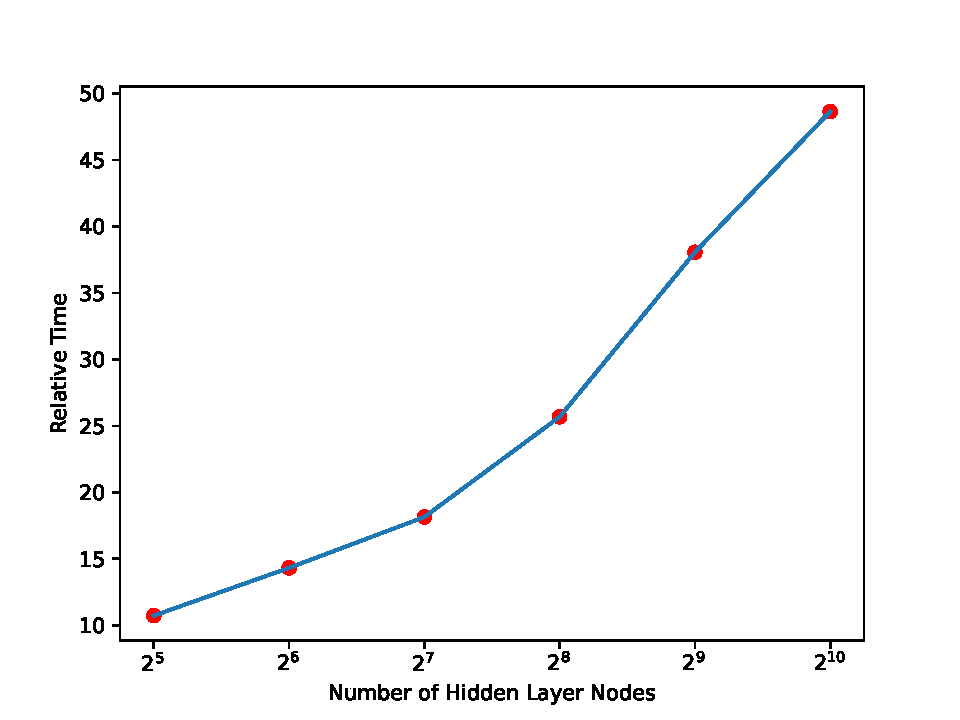
\includegraphics[scale=0.8]{figures/cpu_vs_gpu/cpu_vs_gpu_performance.pdf}
    \caption{The figure shows the relative measured execution time used per sample using $L = 512$ Leapfrog steps,
    as a function of number of parameters. The CPU measurements are done using an 8-core M1 CPU (Apple Silicon). The GPU measurements
    are made with an NVIDIA Tesla P100 GPU.
    }
    \label{fig:relative_performance}
\end{figure}

\subsubsection{Prediction Time}
As we discussed in the introduction, the execution time's order of magnitude when using {\tt Prospino} is in the order of hours. 
If BNNs are to serve as a viable alternative to these calculations, it must at least significantly reduce the time it takes to compute predictions. In figure \ref{fig:prediction_time}, we 
show the average execution time to compute predictions using all models in table~\ref{tab:deep_models}.
For each model, we randomly generated input points of correct dimension and computed predictions for up to 4096 input points simultaneously.
The execution times appear proportional to the number of input points provided for each model, which perhaps is not all that surprising. We can crudely infer by inspection that increasing the order of magnitude by one does the same for the execution time. Still, the order of magnitude for a single input point is at the order of a millisecond which is a significant speedup over {\tt Prospino} calculations. Both the sample mean of the predictions and the sample error is computed during the measurement. The measurements were performed on an M1 Apple Silicon CPU using {\tt perf\_counter} from the module {\tt time} provided by the standard library of Python.

The performance degradation that the computations in figure \ref{fig:prediction_time} suffers is inherently due to the limited vectorization capability of the CPU's computing units when performing matrix multiplications in the forward pass of the individual neural network models. The computation itself is performed with all 1000 sampled networks simultaneously, and so one might hypothesize that more specialized computing units may be able to handle several input points while applying all sampled networks at the same time. As it turns out, GPUs are excel at executing matrix multiplication and even more fortunate, {\tt TensorFlow} has added support for the built-in GPU on Apple Silicon system-on-chips. In figure \ref{fig:prediction_time_gpu} we can see the execution times achieved using the GPU to perform the same computations as before. In this case the order magnitude remains more or less the same in all the tests. Thus, computing predictions on several points can benefit greatly if the execution is employed on a GPU. Note, however, that the measured execution time of ``model 1'' is slightly slower than for more points which likely is due to the overhead introduced by using the GPU for such a simple model. Care must thus be taken when considering what type of hardware the computations should be performed with.

\begin{figure}
    \centering
    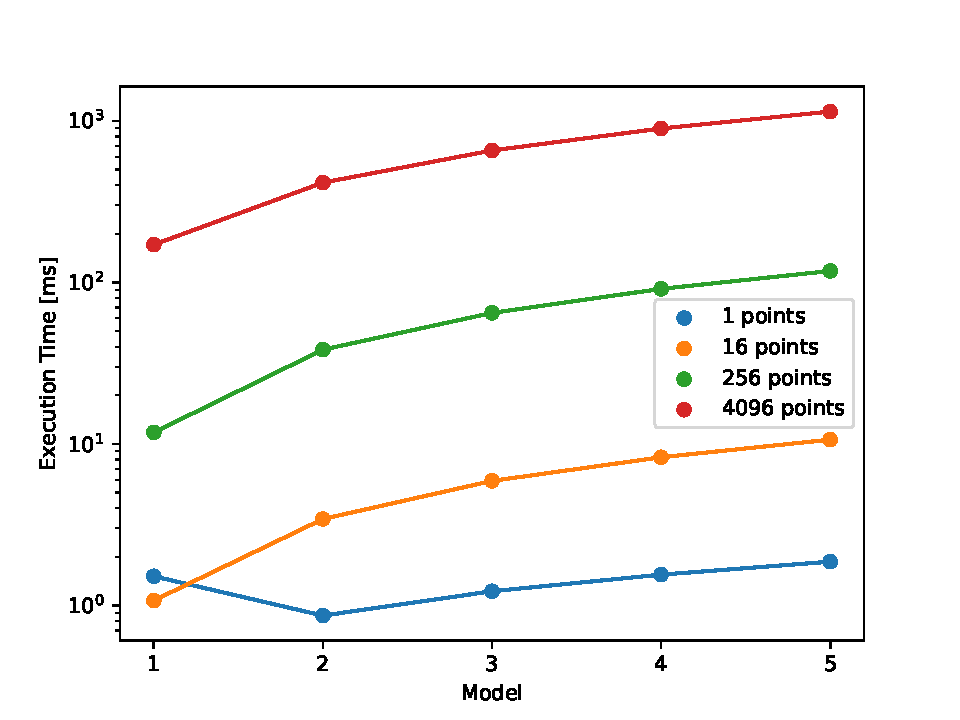
\includegraphics[scale=0.8]{figures/prediction_time/prediction_time.pdf}
    \caption{The figure shows the average prediction time to compute a prediction given a single input $x$ using the models in table \ref{tab:deep_models}. The average time used is measured in ms and is averaged over 1000 randomly sampled points. The measured time includes computation of the sample mean and sample error.
    }
    \label{fig:prediction_time}
\end{figure}

\begin{figure}
    \centering
    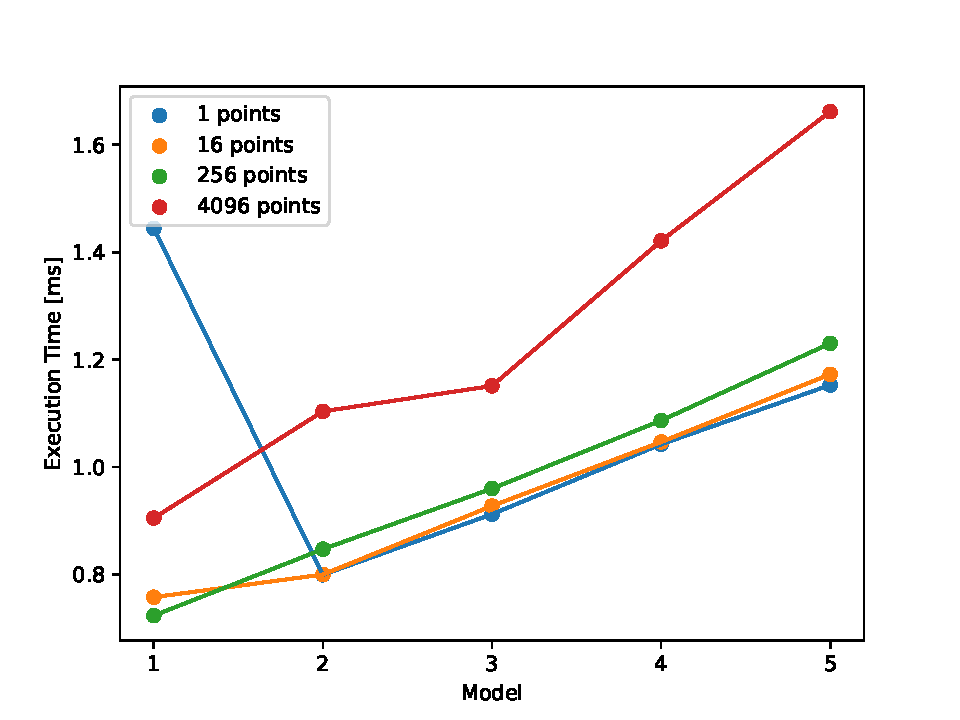
\includegraphics[scale=0.8]{figures/prediction_time/prediction_time_gpu.pdf}
    \caption{The figure shows the average prediction time using the built-in GPU on an M1 Apple Silicon system-on-chip to compute a prediction given a single input $x$ using the models in table \ref{tab:deep_models}. The average time used is measured in ms and is averaged over 1000 randomly sampled points. The measured time includes computation of the sample mean and sample error. 
    }
    \label{fig:prediction_time_gpu}
\end{figure}

\subsubsection{Loading Times}
Even if we have demonstrated a substantial speedup for predictions using BNNs, we have thus far ignored the fact that empirical distribution representing the weights of the BNN is stored on disk which typically means an solid state drive (SSD) with modern computing hardware. The memory bandwidth between the SSD and the faster forms of memory such as RAM, cache and registers becomes a potential bottleneck for performance. Although cache and registers introduce fast memory transfer of stored data to the computing units of the CPU, they typically boast a fairly limited capacity. Thus loading in the entire BNN model might not be viable and we may observe that once we need to models with a large number of parameters, the loading times dominate the computational cost involved with computing predictions. This added computional cost stems from the transfer of data back and forth between the RAM, and the cache and registers. An additional problem is that if the BNN model is simply used for a single prediction at a time, it might simply be loaded a single time before it is dumped from working memory all together. In this case, the initial load may dominate the computational cost all together. 

In figure \ref{fig:loading_times} we show the resulted loading times measured using an M1 Apple Silicon system-on-chip and {\tt time.perf\_counter} from Python. The memory allocated to the BNN models were deallocated manually using the {\tt del} operator provided by Python to ensure that each load of the model of the model was from the SSD. The models loaded in are the ones listed in table \ref{tab:deep_models}. Given the order of magnitude of the loading times displayed in the figure is approximately the same order of magnitude as the execution time, we have demonstrated that BNNs can provide a serious substitute for {\tt Prospino} calculations from a purely computational perspective. It remains to be seen if the predictions themselves are reliable enough for this substitution to be adopted, which we will explore in later sections.

\begin{figure}
    \centering
    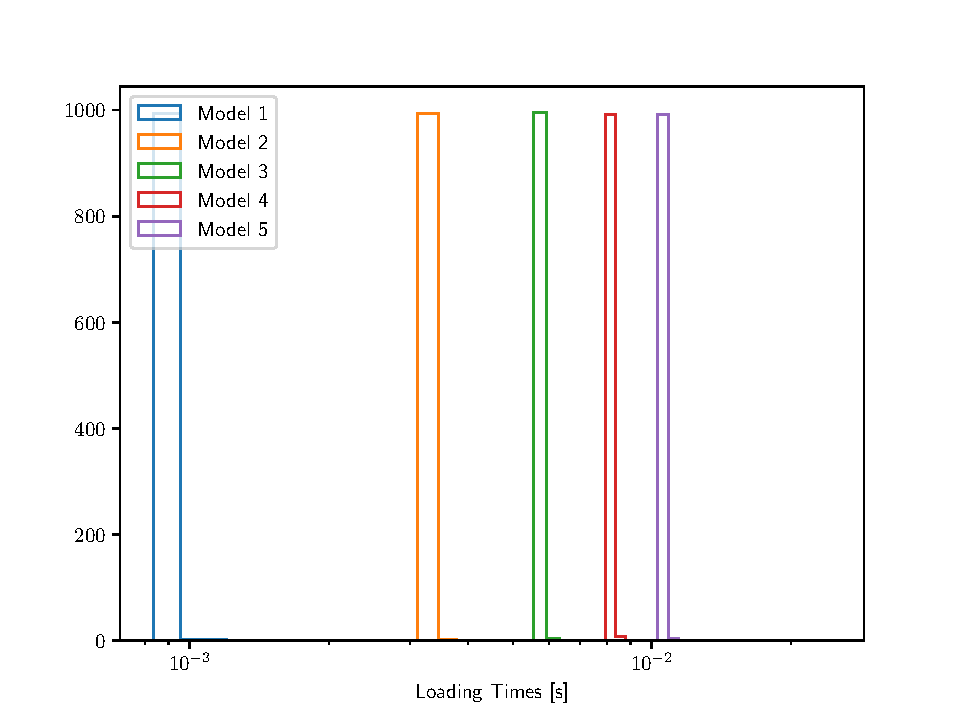
\includegraphics[scale=0.8]{figures/computational_cost/loading_times.pdf}
    \caption{
        The figure shows the histograms of measured loading times in seconds using the models in table \ref{tab:deep_models}. The measurements were performed using {\tt time.perf\_counter} from Python using an M1 Apple Silicon system-on-chip. The time measurements consist of 1000 measurements for each model.
    }
    \label{fig:loading_times}
\end{figure}



\subsection{Posterior Distribution of Weights}
An important problem to consider is if we can even justify the use of Monte Carlo samplers to sample from the exact posterior instead of using the approximation employed by variational inference with a parameterized surrogate posterior which is the most ubiquitous method of training BNNs in the literature. The surrogate distribution is usually a factorized normal distribution of the form
\begin{equation}\label{eq:surrogate_dist}
    q \propto \prod_{i, j, \ell} \mathcal{N}(\mu_{ij}^\ell, (\sigma_{ij}^\ell)^2) \mathcal{N}(\mu_{j}^\ell, (\sigma_{j}^\ell)^2),
\end{equation}
meaning for each parameter in the model, we assume its posterior distribution can be written as an independent Gaussian distribution with a mean $\mu_{jk}^\ell$ and a standard deviation $\sigma_{ij}^\ell$ for the kernels, and $\mu_j^\ell$ and $\sigma_j^\ell$ for the biases. The method sports some fairly obvious advantages like the fact that one can perform \textit{online training}, i.e. continue training once new data becomes available starting from an earlier \textit{checkpoint} by using $q$ obtained during earlier training as the prior. The way we have trained BNNs in this thesis does not permit this form of training because we cannot formulate a prior based on the empirical distribution we have sampled. Thus we cannot use the weights of the model that we have already sampled to continue training. We must start over entirely and discard the empirical distribution we obtained with the prior dataset. 

It has been widely discussed that BNN posteriors are typically found to be multi-modal \cite{google_bnn_posteriors}. We demonstrate this observation in figure \ref{fig:posterior_kernels}.
We can observe that the projection onto the planes shown there indicate that the posterior distribution indeed is multimodal
and unlikely to be approximated well with a parameterized surrogate distribution like the one in eq.~\eqref{eq:surrogate_dist}.

\begin{figure}
    \centering
    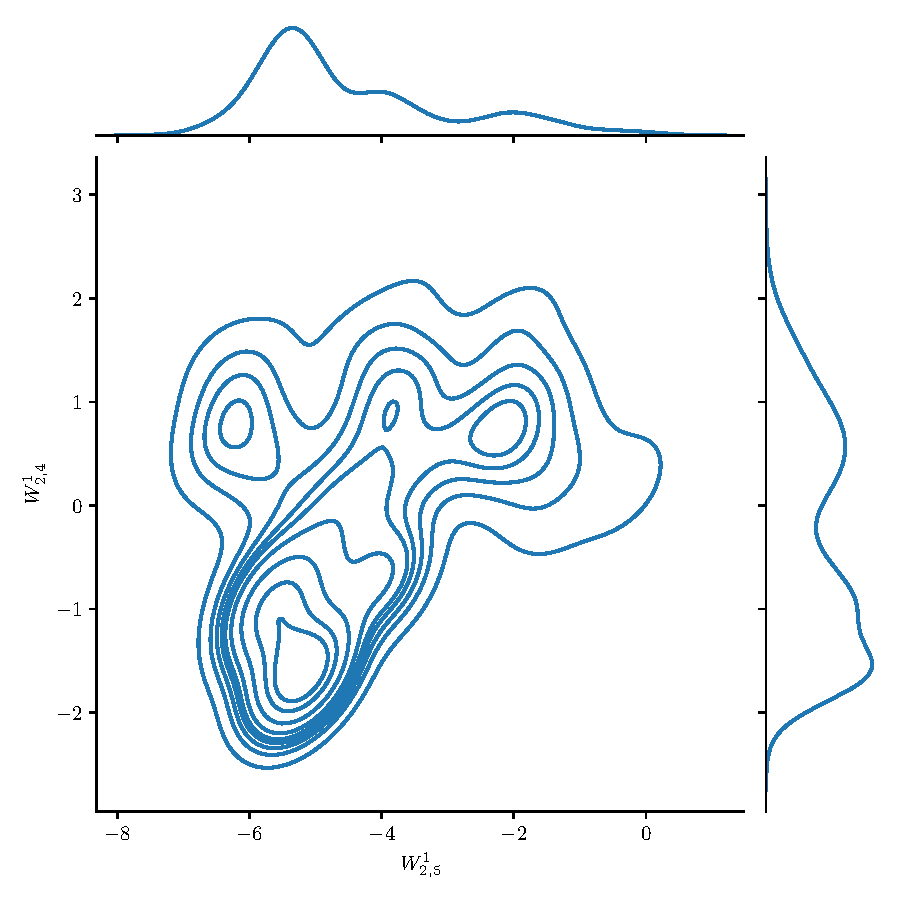
\includegraphics[scale=0.7]{figures/posterior_distribution/posterior_weights1.pdf}
    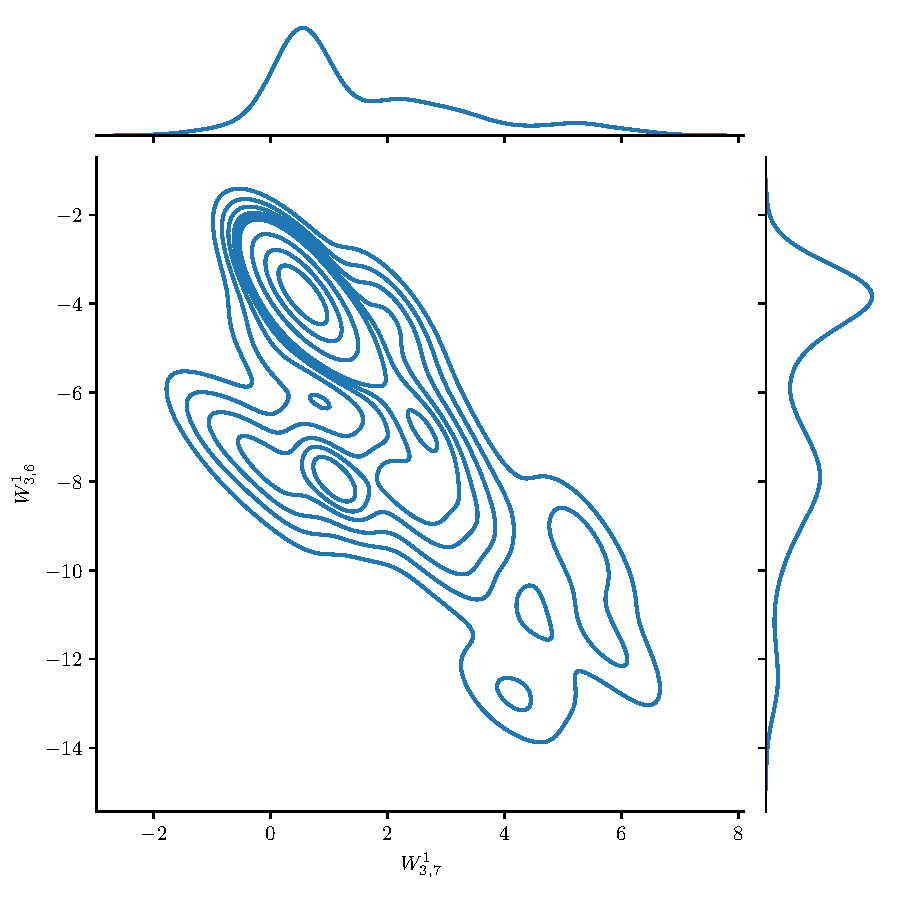
\includegraphics[scale=0.7]{figures/posterior_distribution/posterior_weights2.pdf}
    \caption{The figure shows the projection of the empirical distribution onto the planes spanned by $(W_{2,4}^1, W_{2,5}^1)$ on the left and onto the plane spanned by $(W_{3,7}^1, W_{3, 6}^1)$ on the right, using the samples from model 3 in table \ref{tab:deep_models}. The distributions are approximated using kernel density estimation. 
    }
    \label{fig:posterior_kernels}
\end{figure}


\subsection{Benchmarks of Hyperparameters}\label{subsec:benchmarks}
\begin{figure}
    \centering
    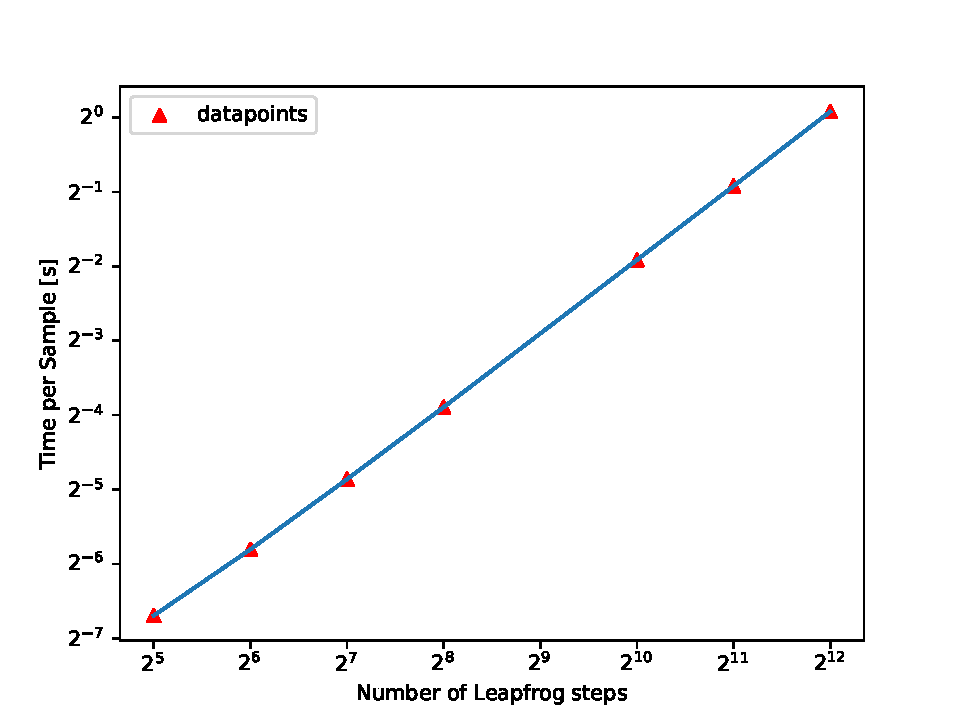
\includegraphics[scale=0.7]{figures/computational_cost/time_vs_leapfrogsteps_hmc.pdf}
    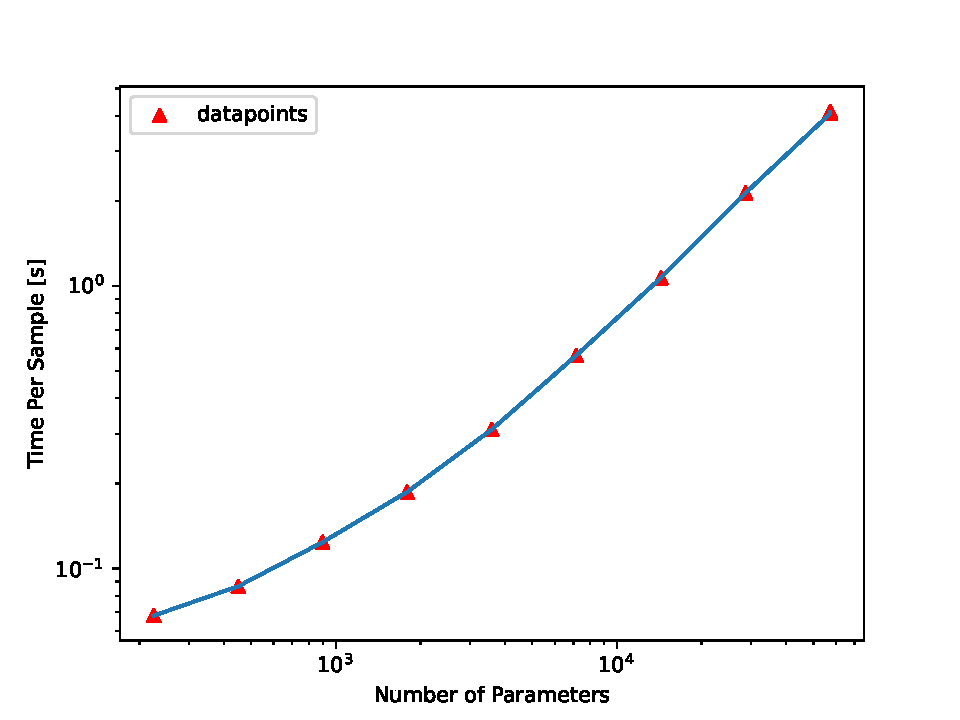
\includegraphics[scale=0.7]{figures/computational_cost/time_vs_params.pdf}
    \caption{The figure at the top shows the measured time in seconds per sample using HMC as a function of Leapfrog steps $L$ using a model with
    561 parameters. The figure at the bottom shows the time in seconds per sample with the same sampler with a fixed number of Leapfrog steps $L = 512$ as a function of number of parameters in the BNN model.
    }
    \label{fig:time_vs_leapfrogsteps}
\end{figure}

\subsubsection{The Effect of Number of Burn-in Steps and Step Size Adaptation}
As we discussed in section \ref{sec:practical_bnn}, we must set a predetermined number of warm-up steps, i.e. number of burn-in steps and number of adaptation steps when using {\tt TensorFlow Probability}'s samplers.
Conventional wisdom would have us believe that increasing the number of burn-in steps increases the probability that the Markov chain has converged
to the stationary distribution of the posterior. Moreover, the literature has shown that NUTS performs at least as good as or better than HMC with an equivalent number of maximum Leapfrog steps or more as the results in \cite{nuts} demonstrated. In our case we have split the number of warm-up steps to 20\% burn-in steps and 80\% adaptation steps, respectively. This is a heuristic recommended by the {\tt TensorFlow Probability} developers.
In figure \ref{fig:standardized_residuals_vs_burn_in_steps} we demonstrate that the claims above may not be general enough to apply to BNNs as the HMC performs better almost regardless of how many burn-in/adaptation steps that are performed. When using NUTS, the performance of the model trained with a substantial amount of burn-in/adaptation steps appear to degrade as opposed to improve. The standardized residual of HMC lies consistently inside the Normal distribution for the most part, while the NUTS sampler produced few models that achieve the same. These results, then, actually indicate that we may be better off running the training procedure of BNNs with a fixed $L$, only adapting the step size. Even better, we may get by with a fairly limited amount of burn-in/adaptation steps and a fairly small $L$. The results in figure \ref{fig:standardized_residuals_vs_burn_in_steps} were generated with a fixed $L = 512$ Leapfrog steps when using the HMC sampler, while the NUTS sampler allowed for a maximum of $L = 4096$ Leapfrog steps. In figure \ref{fig:avg_leapfrog_steps_vs_burn_in}, we show the average number of Leapfrog steps the NUTS sampler used during the generation of the Markov chain as a function of number of warm-up steps.


\begin{figure}
    \centering
    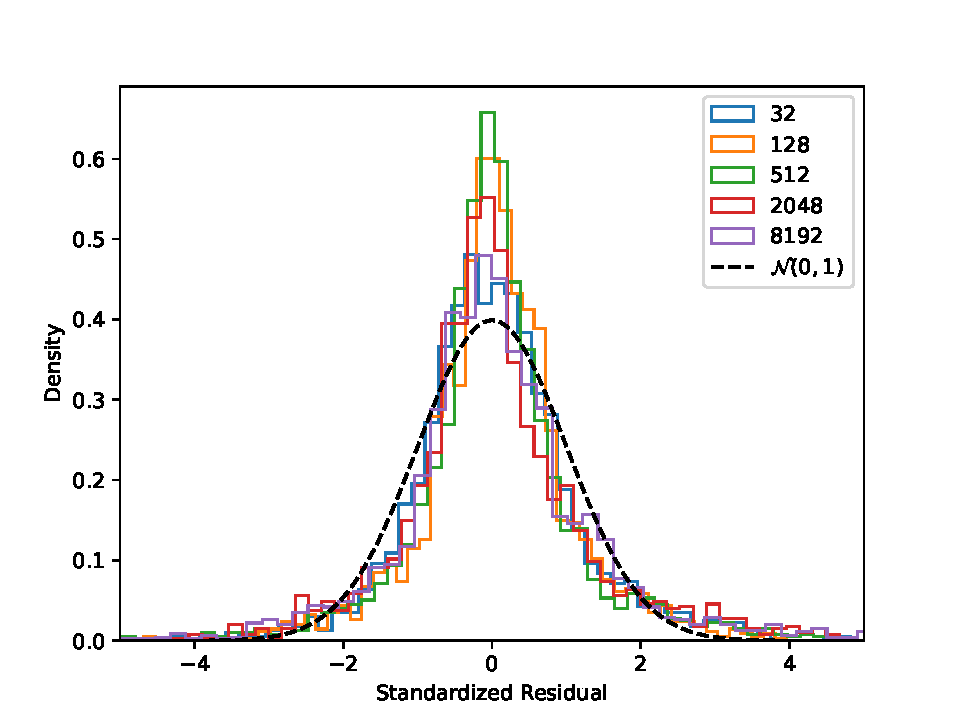
\includegraphics[scale=0.7]{figures/standardized_residuals/effect_of_burnin/standardized_residuals_hmc_vs_burn_in_steps.pdf}
    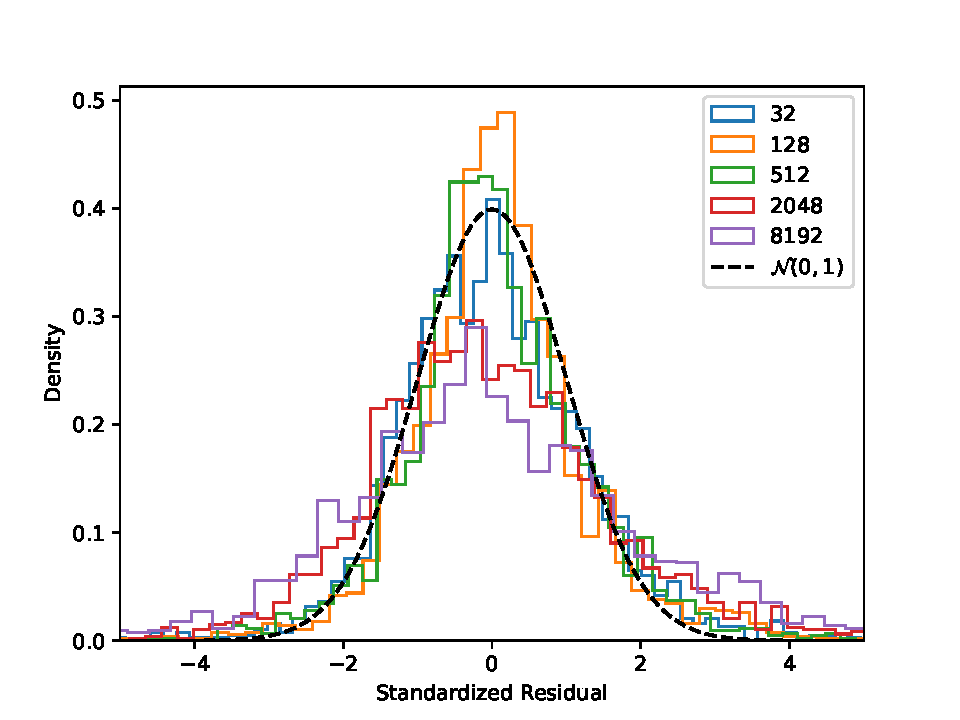
\includegraphics[scale=0.7]{figures/standardized_residuals/effect_of_burnin/standardized_residuals_nuts_vs_burn_in_steps.pdf}
    \caption{The figure shows the standardized residuals computed on the testset. The model architechture used is a model with layers 5-20-20-1 with $\tanh(x)$ as the hidden activation function. In the top figure, we have used the HMC sampler with a fixed number of Leapfrog steps $L = 512$. In the bottom figure, we have used the NUTS sampler with a maximum tree depth of $12$ corresponding to a maximum of $L = 2^{12} = 4096$ Leapfrog steps. The remaining important hyperparameters were 2500 pretraining epochs with a batch size of 32 using the ADAM optimizer. In total a 1000 neural networks were sampled in each case with a thinning-amount of 10 steps between each sample.
    }
    \label{fig:standardized_residuals_vs_burn_in_steps}
\end{figure}


\begin{figure}
    \centering
    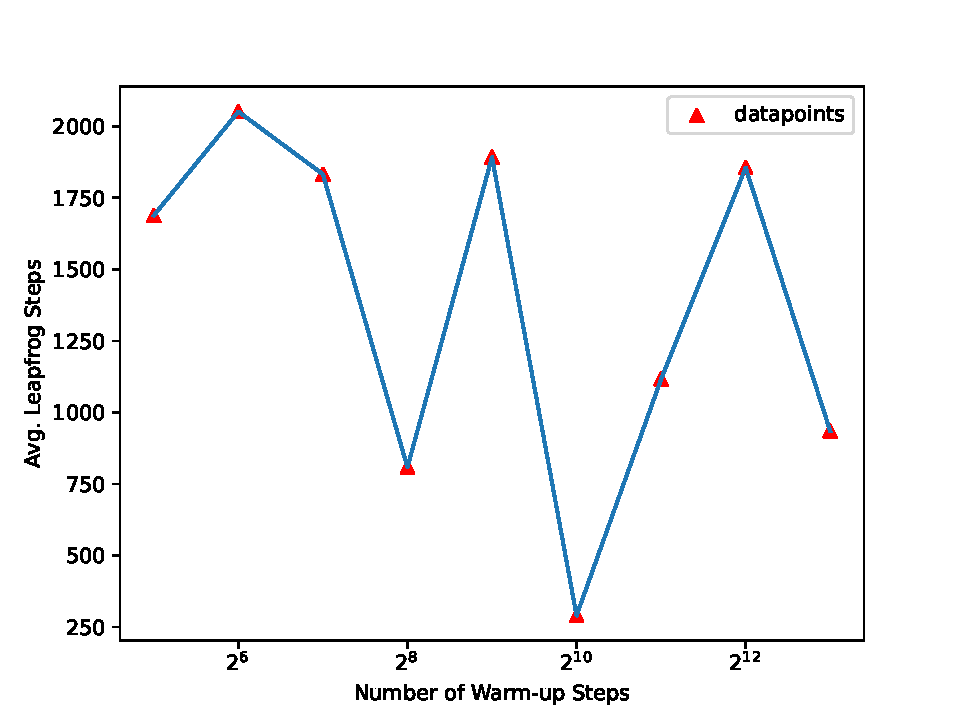
\includegraphics[scale=0.8]{figures/standardized_residuals/effect_of_burnin/avg_burnin_steps_nuts_vs_burn_in_steps.pdf}
    \caption{The figure shows the average number of Leapfrog steps $L$ as a function of number of warm-up steps used by the NUTS sampler when sampling the models shown in the bottom of figure \ref{fig:standardized_residuals_vs_burn_in_steps}. We have included a few more measurements to showcase how fluctuating the average number can be. 
    }
    \label{fig:avg_leapfrog_steps_vs_burn_in}
\end{figure}




\subsubsection{The Effect of Pretraining}
Pretraining a model before initiating the Markov chain is typically suggested as a means to accelerate convergence to the stationary distribution by minimizing a selected loss function with respect to the model parameters to obtain a point estimate. The point estimate is then used as the initial point of the Markov chain. This may help but as we discussed in chapter \ref{chap:mcmc}, the typical set, the set which we seek to sample from, may not lay particularly close to the mode of the loss function, or as we know it as, the potential energy function. Thus we have good reasons to challenge this recommendation and verify that it indeed improves the performance of the BNN models we sample. In figure \ref{fig:std_residual_vs_pretraining}, we
show the computed standardized residuals resulting from models trained with a varying amount of pretraining. Here all other
hyperparameters are fixed. The figure demonstrates a pretty noticable improvement as the amount of pretraining increases, up to a point. Once we surpass 2048 epochs of pretraining, we see a slight degradation of the model performance with a larger spread in the residual distribution. But we can rest assured that pretraining can be used to increase the performance of the trained BNN when everything else is held fixed. The various hyperparameters used are listed as part of the figure to avoid tedious repetition.


\begin{figure}
    \centering
    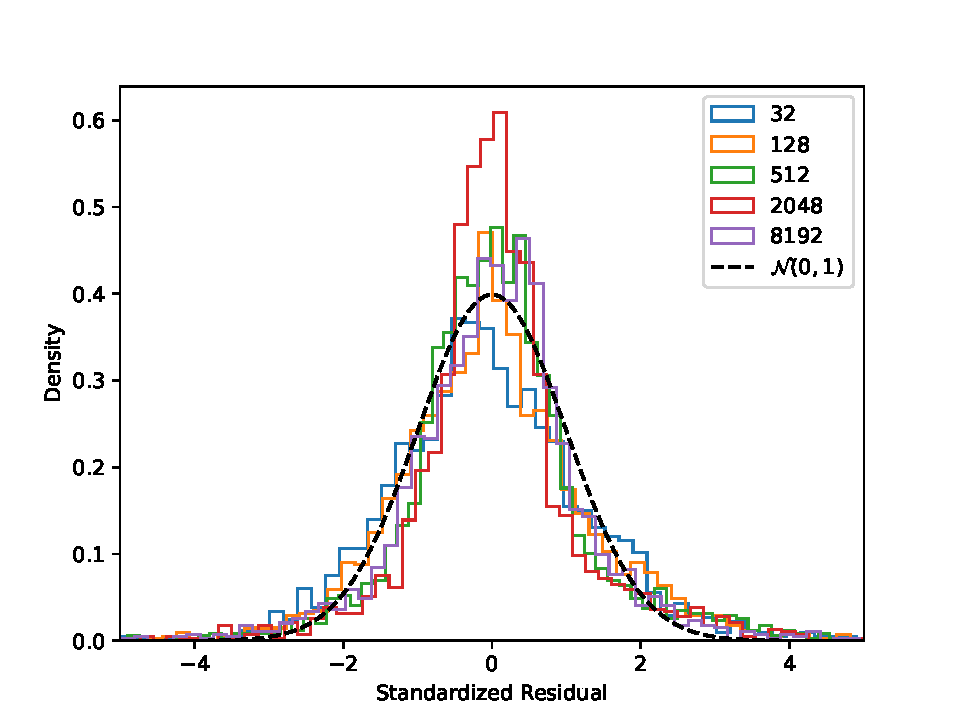
\includegraphics[scale=0.8]{figures/standardized_residuals/effect_of_pretraining/standardized_residuals_hmc_vs_pretraining_steps.pdf}
    \caption{The figure shows the standardized residuals of a model with the architecture 5-20-20-1 with $\tanh(x)$ as the
    hidden activation function. In this case the varying number of the number of epochs run with pretraining starting from 32 all the way up to 8192. The batch size used was 32, the number of warm-up steps was 1000 (200 of which were burn-in steps and 800 were adaptation steps). We fixed the Leapfrog steps to $L = 512$ using the HMC sampler. The ADAM optimizer was used for the pretraining phase. As usual we sampled 1000 neural networks with 10 steps between each sample.
    }
    \label{fig:std_residual_vs_pretraining}
\end{figure}

\subsubsection{Effect of Number of Parameters}
Increasing the number of parameters of the BNN model may help capture the underlying model from the data to a larger degree. The typical problems posed by the \textit{bias-variance trade-off} \cite{ml_for_physicists} (pages 12-13) does not play as significant a role here since the trained model can compute a sample variance along with its prediction. This does not mean it is immune, however, as the model will still sample according to the nuances found in the training data which in principle may be due to noise. As explained in section \ref{sec:perf_metrics}, the dataset produced by {\tt Prospino} contains very little noise and thus specializing the model to inherent noise is not the issue. Instead, we may be a bit unfortunate with the splitting of the dataset such that the training data itself contains information in some of its datapoints that are not present in the test data or vice versa. This may result in a model with a large set of parameters that produces poor results when generalizing to the unseen test data. Moreover, the dataset we use is fairly small (~ 16000 datapoints in total), which may exacerbate the overfitting effect.
In figure \ref{fig:standardized_residual_vs_params}, we show the computed standardized residual distribution of the models listed in table \ref{tab:deep_models}, which gives us an idea of the performance the BNNs have on this dataset as a function of the number of parameters. We can note that model 3 and 4 performs fairly well given our chosen benchmark measure, but that model 5's performance degrade somewhat, which is the model that contains the most parameters of the models tested. 

\begin{figure}
    \centering
    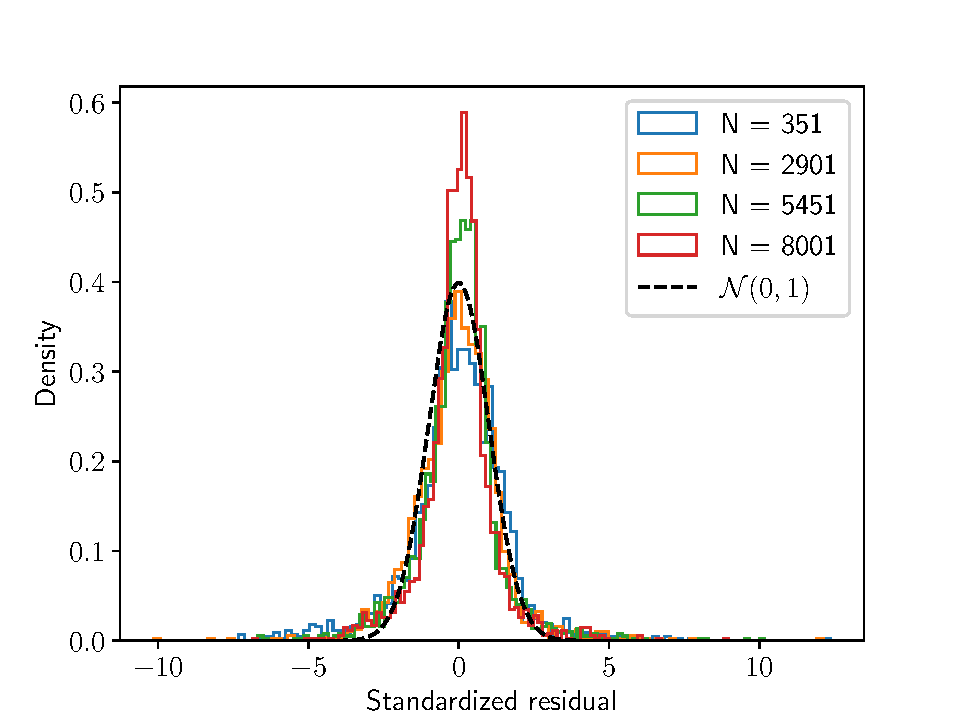
\includegraphics[scale=0.8]{figures/standardized_residuals/standardized_residual_simple_models.pdf}
    \caption{
        The figure shows the distribution of the standardized residuals computed on the test data using the models listed in table \ref{tab:deep_models}. The Normal distribution is drawn in with a dotted black line for benchmarking reference.
        The figure is meant to illustrate the performance of the models with respect to the number of parameters in the models.
        The models were trained with 2500 warm-up steps (20\% burn-in and 80\% adaptation), gathering 1000 neural networks with 10 steps between each sample. We used 1000 pretraining epochs with a batch size of 32. The kernel used was the NUTS kernel with a maximum of $L = 4096$ Leapfrog steps. 
    }
    \label{fig:standardized_residual_vs_params}
\end{figure}


\subsection{Neutralino-Neutralino Cross Sections}\label{subsec:neuralino_experiments}
\subsubsection{Predictive Distributions}
As we discussed in chapter \ref{chap:bayesian_ml}, one of the primary objects we seek to compute
in Bayesian ML is the predictive distribution $p(y^*|x^*, D)$ for a target $y^*$ given an unseen input point $x^*$ and
a training dataset $D$. In figure \ref{fig:predictive_distributions}, we show the predictive distribution computed with model 3 in table \ref{tab:deep_models}. In the figure on top, the sample mean approximates the true target well with a fairly small spread in the distribution which is a desirable outcome in most cases. There are, however, ill cases as well which we demonstrate in the figure at the bottom. Here the true target lies entirely outside the predictive distribution. Thus care must be taken to understand when a BNNs prediction is reliable and when it is not.
\begin{figure}
    \centering
    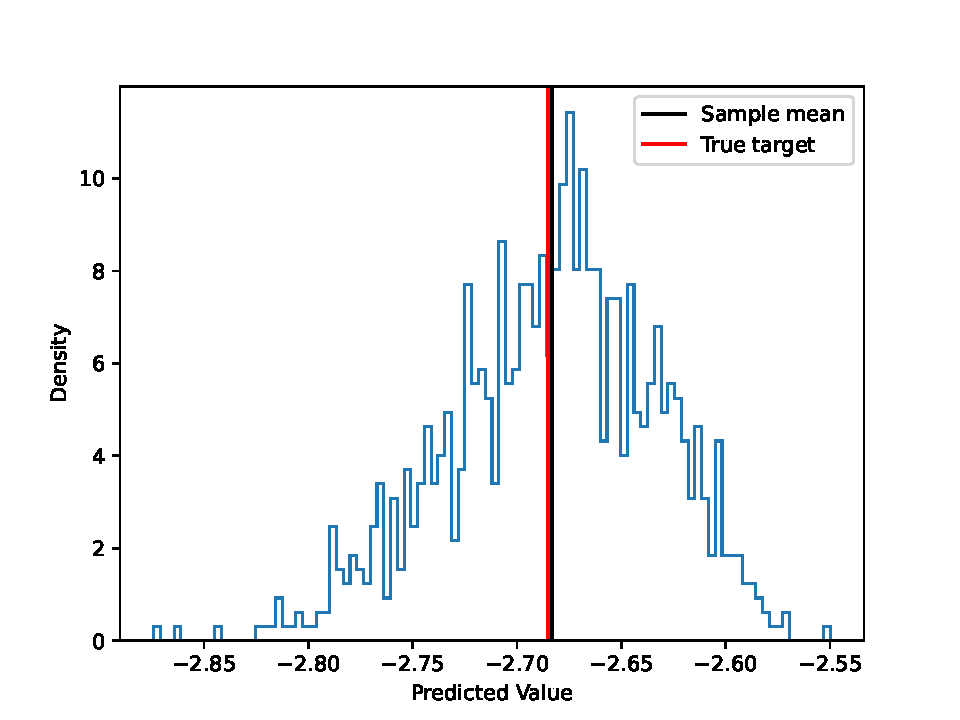
\includegraphics[scale=0.7]{figures/predictive_distributions/predictive_distribution_point_idx_360.pdf}
    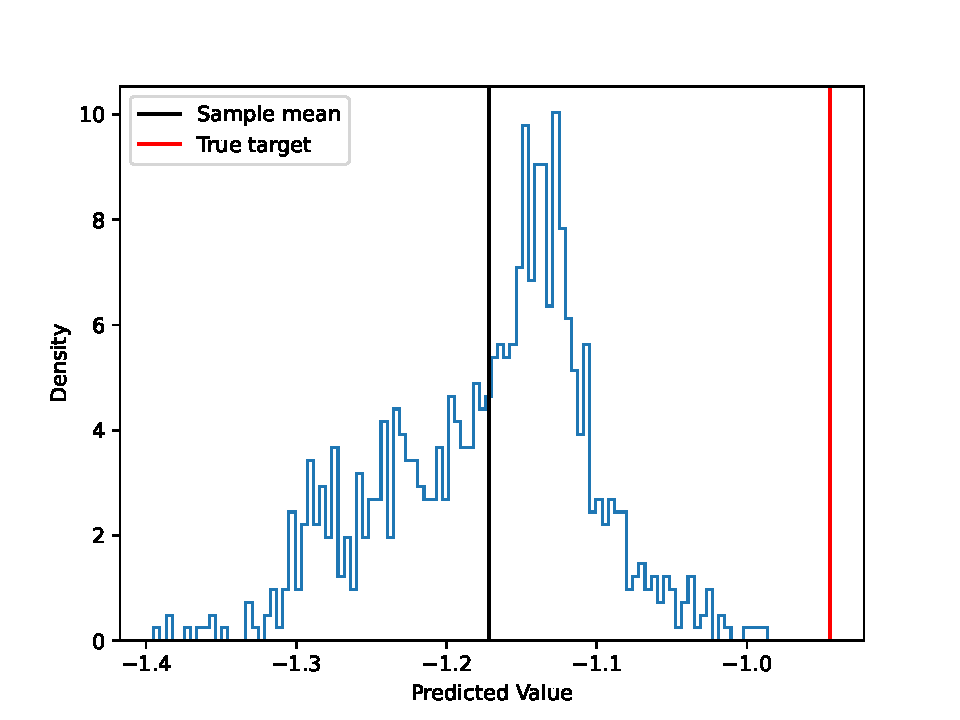
\includegraphics[scale=0.7]{figures/predictive_distributions/predictive_distribution_point_idx_2052.pdf}
    \caption{
        The figure shows the predictive distribution estimated by use of model 3 in table \ref{tab:deep_models} for to randomly chosen points from the test set. The red line shows the true target and the black line shows the predicted sample mean obtained from the distribution. The figure on top demonstrates a case where the sample mean is approximately the same as the target, while the figure at the bottom demonstrates a case where the true target lies entirely outside the predictive distrbution. 
    }
    \label{fig:predictive_distributions}
\end{figure}



\begin{table}[h!]
    \centering
\begin{tabular}{c@{\hspace{1cm}}c@{\hspace{1cm}}c@{\hspace{1cm}}c@{\hspace{1cm}}c@{\hspace{1cm}}c}
\hline
    Burn-in steps & \makecell{Number \\of \\steps between} & Kernel & \makecell{Number \\ of \\ results} & \makecell{Pretraining \\ epochs} & \makecell{Pretraining \\ batch size} \\
\hline
    2500 & 10 & NUTS & 1000 & 1000 & 32 \\
\hline
\end{tabular}
\caption{
    The table shows the training configuration used to sample the models listed in table~\ref{tab:deep_models}.
}
\label{tab:NN_mse_scores}
\end{table}



